% Here is a suggested template for PhD research proposal for the
% first annual report.
% Written originally 2010-06-22 by T. W. Yee.
% Last modified      2010-07-22 by T. W. Yee.


\documentclass[12pt,a4paper]{article}


 \usepackage{natbib}    % For BibTeX
 \usepackage{graphicx}  % To import .pdf files
 \usepackage{booktabs}
%\usepackage{times}
 \usepackage{setspace}
 \onehalfspacing

 \oddsidemargin  -10mm
 \evensidemargin -10mm
 \headheight 0mm
 \headsep -3mm
\textheight 250mm
\textwidth 180mm
\topmargin -4mm
\topskip -10mm

%\textwidth=450pt
%\hoffset=-2cm

\usepackage[hidelinks]{hyperref}

\begin{document}

\begin{Large}
\begin{center}
\textbf{Better Prediction of Bus-time Arrival} \\
\textbf{by Tom Elliott} \\
\textbf{for a PhD in Statistics}
\end{center}
\end{Large}


\hfill{Student ID: 1596870}

\hfill{Email: tom.elliott@auckland.ac.nz}

Supervisor: Professor~T.~Lumley

% Co-supervisor: Dr~B.~Brewer

% Advisory Committee: Drs~B.~Efron, D.~R.~Cox, K.~Pearson.\footnote{
% Specify the affiliation if outside the UoA Statistics
% Department.}



\begin{center}
\today
\end{center}


This document represents the student's research proposal after
one year of provisional PhD registration.
Confirmed PhD registration is now sought.




% ----------------------------------------------------------------------
\section{Introduction}
\label{sec:intro}



% This document is a template that can be edited by the student.
% Fill in the details as you go along and delete these instructions.
% Do have your research proposal scrutinized by your supervisor before
% submitting it to the department.



% Give a few paragraphs here on the general background
% to your research proposal; put the full details in
% Section~\ref{sec:background}. You might want to cite a few
% previous important results/papers. Describe any theory briefly
% here but put most of the details in Section~\ref{sec:background}.
% Describe any data in general with a few lines here but put the
% full details in Section~\ref{sec:data}.


% Motivate this section well \ldots why is the topic important?
% What use will the thesis have?
% What is unknown that will be known upon completion?


% This section should be understandable by an intelligent person
% who is not familiar with the technical details involved.
% The reader should be convinced that your work
% is worthwhile.





% Some of our PhD students have published in the primary literature
% directly using material from their thesis,
% e.g.,
% \cite{wors:1979},
% \cite{yee:wild:1996},
% \cite{wild:yee:1996},
% \cite{murr:1999},
% \cite{jian:scot:wild:2006},
% \cite{roev:meye:etal:2007},
% \cite{mill:stew:2007},
% or submitted such as
% \cite{lee:hiro:2008}.
% Ideally you should aim at least one of your publications towards
% a mainstream statistics journal, preferably your first one.
% All publications should be in a peer-reviewed international journal.
% It should be in the primary literature.
% Statistical theory and methodology is to be regarded as the highest
% form of quality output.
% Accompanying high quality software that can easily be used
% by others (such as a R package) is also good.
% It is best to submit to journals before the completion of a thesis
% because an acceptance validates the quality of that research.



% A word about writing up your thesis.
% In general, the Department of Statistics recommends \LaTeX{} rather than
% Microsoft Word.
% \LaTeX{} is easily run on the Department's Linux machines.
% A website that converts pdf into Word is \textsf{www.pdftoword.com}.
% The University of Auckland offers a half-day workshop
% on \LaTeX{} to postgraduate students.
% There is Sweave \citep{lmucs-papers:Leisch:2003b} which allows R
% \citep{R:Ihaka+Gentleman:1996} to be embedded into a \LaTeX{}
% document, and so the output does not have to be manually
% cut-and-pasted in. Sweave is useful for presentations too,
% in conjunction with Beamer.


% There is an editor called Emacs which is useful for all types of
% editing, including \LaTeX{}, C, and R.
% In Windows there is Tinn-R for R files and MiKTeX for \LaTeX{}.


% Note that {BibTeX} items are available from MathSciNet
% which is part of the ``Library Databases'' in the UoA electronic library
% system.
% There is a close relationship between EndNote and {BibTeX}.




In many cities, public transport is important to management and traffic etc.
For commuters, knowledge of expected waiting times is useful for both trip planning,
as well as reducing frustration at waiting for long periods of time.


Over the years, many technologies have been added to transit vehicles---such as 
automatic vehicle positioning (AVL) systems---which are used to provide commuters with
up-to-date information on the location and, more importantly, expected arrival time of their bus.


Many applications have been produced to present this information to commuters, and many different methods
for generating this information have been used.
Notable methods are the Kalman Filter \citep{cathey-dailey:2003}, \ldots


The main problem is efficiency.
The resulting algorithm must be able to update the predictions quickly, 
to reduce the time between receiving a vehicle location, and getting predictions to commuters.
This can be difficult when there are a lot of busses (the Auckland Transport service has up to $N$ 
busses operating simultaneously at peak traffic times).
Additionally, new locations are recieved every 10--30~seconds, 
so the predictions will constantly need updating as new information arrives.



Additionally, the predictions supplied to commuters can be terribly inaccurate.
In the Auckland Transport system, common phenomena include ``time travelling busses'', 
where the ETA increses significantly (from, for example, 5~minutes to 15~minutes), 
or ``disappearing busses'' that display a realistic ETA, leading to ``DUE'', 
and finally removed from the board without the bus having gone past.



% ----------------------------------------------------------------------
\section{Background}
\label{sec:background}


% Background knowledge is crucial, therefore describe it fully here.
% Specify the background to the problems you are trying to solve.
% Define anything technical that most statisticians will not be
% familiar with.


% What previous work has been done in the area?
% Cite references relating to such work, e.g.,
% in the form of \cite{reid:2003} and \cite{efro:tibs:1993}.
% Has anybody described any open problems in the literature?


% Make sure that problems arising from the background knowledge
% are clearly described. There should be a logical flow of thought
% in this section starting from the background and leading to the
% problem on hand.




% Don't put anything new in this section.


Accurate prediction of bus arrival (or departure) time from bus stops is dependent on many components.
The primary component is the AVL system used to track the real-time positions of vehicles.
A statistical model is then applied that uses this AVL data to model the movement of the bus over time. 
Using this model, predictions of arrival/departure time can be made.


There are many forms of AVL, although the most common (and the one we will be working with) is GPS.
In this, each AVL report contains the time, vehicle information (identification, possibly trip and/or ``block'' ID,
and the GPS coordinates).

Google has standardised the AVL system into GTFS\footnote{\url{https://developers.google.com/transit/gtfs/}}, 
which means any applications should be transferrable to any 
public transport system using GTFS (Auckland Transport does, along with $M$ other companies worldwide).
GTFS has two components: \emph{realtime} (live positioning information) and \emph{static} (schedule information,
route shapes, timetables, etc).


With an accessible\footnote{so long as AT makes the data available} data format, the main focus will be on algorithms
used to model and predict arrival times. The Kalman Filter is one commonly used method for this, and has been used
in many applications such as \cite{cathey-dailey:2003}, \cite{cn}, and \cite{cn}.
The main idea behind this algorithm is that it is \emph{fast}: it only involves matrix operations and works with 
the mean and variance of a normal distribution.
No complex integrations of MCMC sampling is required.


The KF algorithm works as follows \ldots

Other modelling methods have been used, such as
nearest neighbour regression \citep{chang-etal:2010},
artificial neural network (AVN) \citep{jeong-rilett:2005}, and
support vector machines (SVN) \citep{yu-etal:2006,yu-etal:2010,yu-etal:2011}.

While the KF algorithm is fast and easy to use, it is limited in its assumption of normality. 
There are multiple extensions of the KF, including the Extended Kalman Filter for using general functions, 
and Particle Filters, which are far more flexible but require significantly more computational power.

Particle Filtering, in the simplest of terms, requires a set of ``imaginary'' points---let's call them imaginary busses.
Each of these is manipulated using the likelihood information to complete the \emph{prediction} step,
which is easy enough.
After prediction, the data is obtained and the likelihood of each virtual bus is computed,
and a new sample is taken (with replacement) with sampling probability proportional to likelihood.
That is, the imaginary busses closes to the real bus are sampled more often, 
and those far away are samples less (or not at all).

The PF can get very computationlly demanding, but it has one great advantage:
the KF filter requires the reported GPS location to be mapped to the trip shape;
the PF does not.
The PF can compare imaginary GPS locations to the true GPS location, and use a bivariate normal distribution
to estimate the likelihood (GPS's have an associated error, so we can use this or estimate it from the data).












% ----------------------------------------------------------------------
\section{So What's New?}
\label{sec:whatsnew}



% List \textit{specific} and \textit{new} results that your thesis
% plans to obtain, especially with regard to new statistical theory
% and methodology.
% It is essential that you have provided comprehensive background
% (in Section~\ref{sec:background})
% so that it is clear what new contributions will be made (here),
% and how they will extend what is currently known.
% Tie these with Appendix~A(i), and a list such as below is a
% good idea.


% For example, all of the points below are new (to my knowledge)
% and have not been done yet.
% \begin{enumerate}

% \item
% Develop a new method for quantile regression based on the
% asymmetric Laplace distribution and the concept of link functions
% and parallelism assumptions (via constraint matrices).


% \item
% Derive the asymptotic properties of the above method,
% both as $n \rightarrow \infty$ and as $p \rightarrow \infty$.




% \item
% Conduct a small simulation to check the mean squared error and
% other properties. To be done in R with some sections written in~C
% calling LINPACK \citep{dong:bunc:mole:stew:1979} for additional speed.



% \item
% Compare my results to those of~\cite{wei:carr:2009}, especially
% relating to boundary effects and small-sample properties.



% \item
% Tackle an important dataset or problem that no one has
% satisfactorily resolved before. It is essential that new
% methodologies are investigated and that novel insights are
% obtained. Note that a conventional analysis, even of a very large
% dataset, is \textit{not} PhD-level research.


% \end{enumerate}




\begin{enumerate}
\item 
  We're going to implement a Particle Filter to model the busses,
  and compare it to the KF (and other methods we can get working or compare with).


\item 
  Then we're going to investigate better summary statistics.
  The mean is great, but only if the posterior is normal.
  It probably wont be, so maybe the median, or mode, or something else, will be better.
  Also, prediction \emph{intervals}! Is the bus 2--3~minutes away, or 2--10~minutes away???

\item 
  Then we will use as much data as possible and see if it improves predictions 
  (like, ``realtime'' congestion data from other busses, historical data, \ldots).

\item 
  Then we want to apply the methods to a real data set (Auckland Transport PTS).

\item 
  And then make it available via the web and/or a phone app.

\end{enumerate}







% ----------------------------------------------------------------------
\section{Data and Special Needs}
\label{sec:data}


% Almost all Statistics PhD theses should analyse at least one
% data set, even if it is a toy data set.


% State their source fully.
% If new data is important to the thesis describe what's new.
% Why is this data set important?
% What is novel about it?
% Specify any ethics or confidentiality issues.


% A plot of some of the data may be useful;
% see Figure~\ref{fig:myfig}.


% Do you have any special needs such as IT needs?
% These include hardware (supercomputing facilities),
% and expertise/technical knowledge.
% Often extra large data sets have special needs associated
% with its processing.
% How do you invisage those needs to be met?



% Funding: anything to report here?
% If your thesis work involves experiments, travel or special
% resources in order to collect data, or essential collaboration with
% experts in your field, then you should describe these requirements
% here along with how you, or your supervisor, will fund these
% requirements. Departments work on tightly planned budgets and
% generally do not have the facilities to pay for unplanned PhD
% related expenses.



% If ethics approval(s)/permissions is needed then put
% any details here.





% \begin{figure}[tt]
% \begin{center}
% %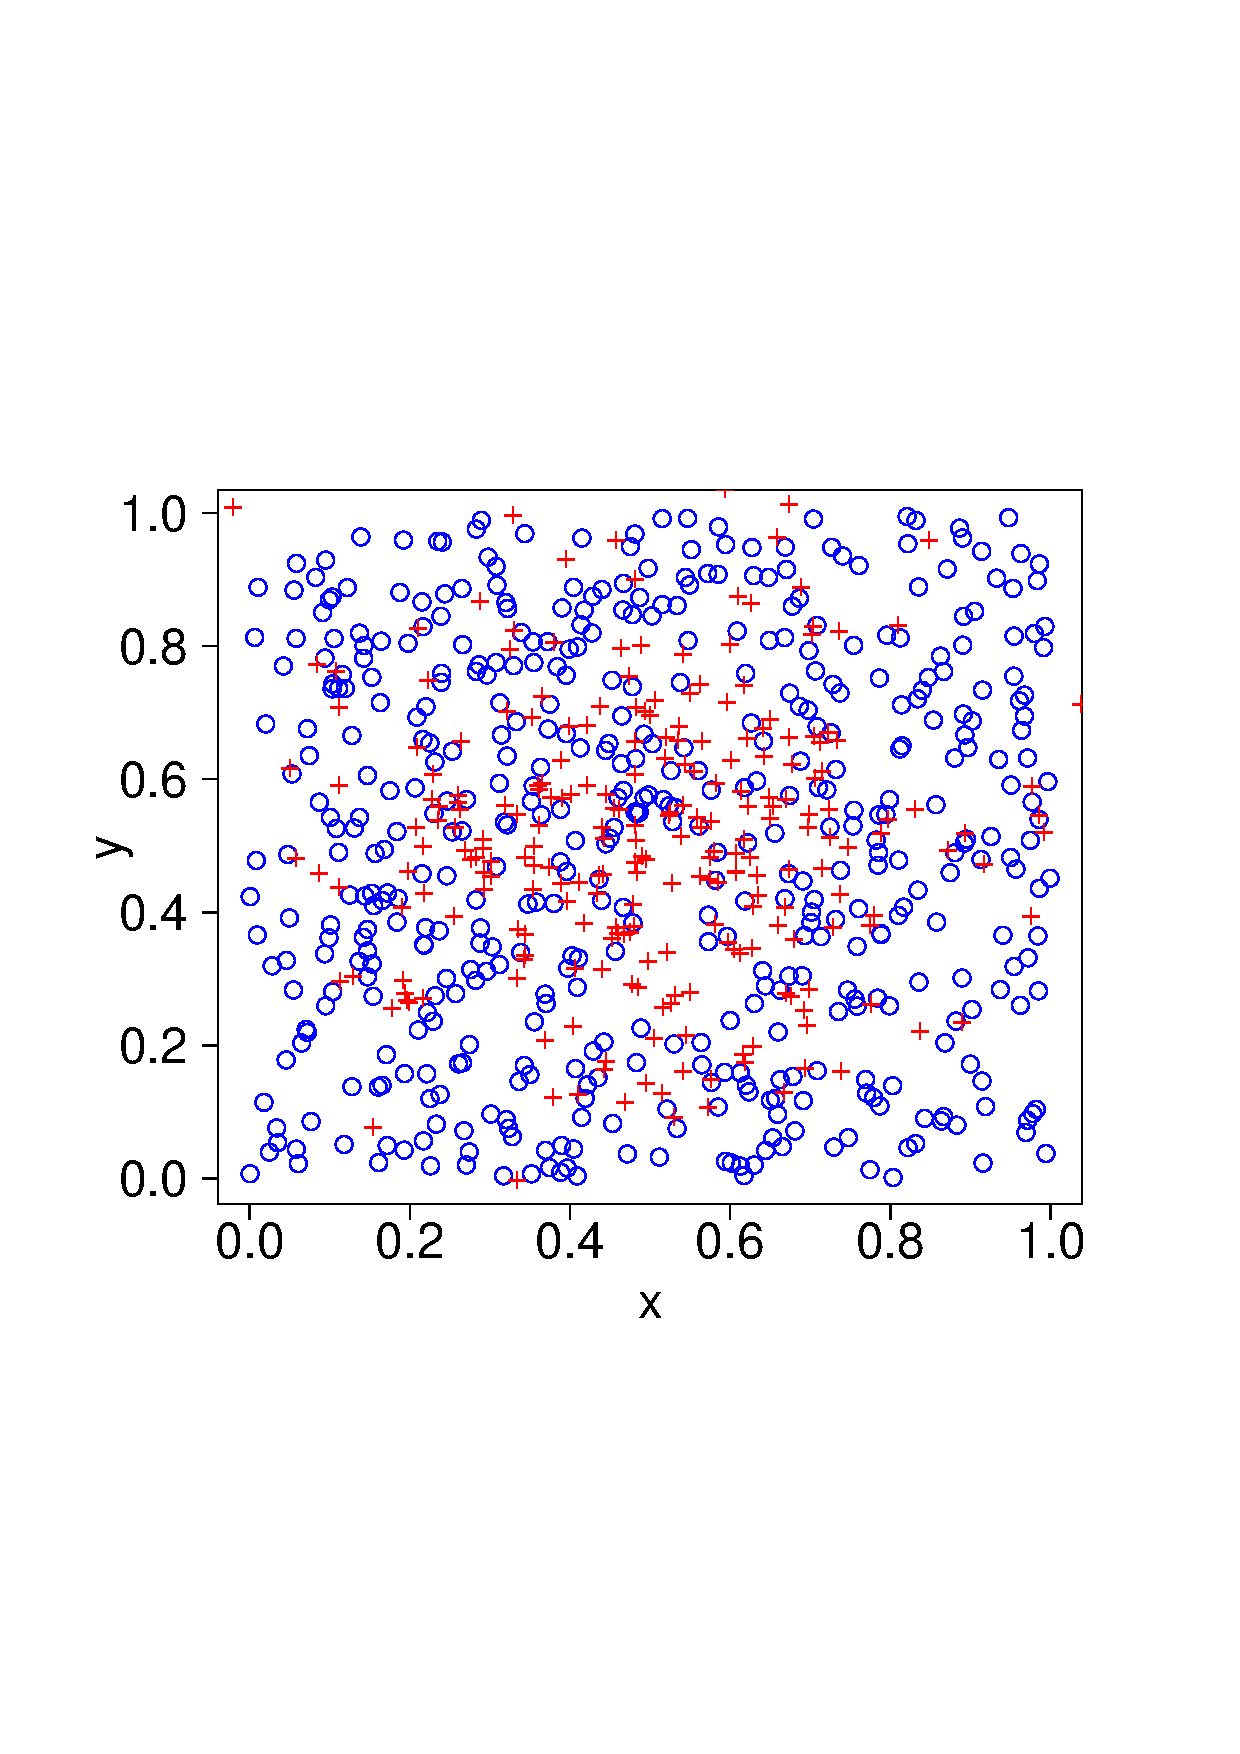
\includegraphics[height=70mm]{./myfig.pdf}
% \caption{
% Data for a two-class classification problem.
% The red ``+'' is for class~1, and $n = 250$.
% The blue ``o'' is for class~2, and $n = 500$.
% }
% \label{fig:myfig}
% \end{center}
% \end{figure}



We will need access to a GTFS realtime feed.
There a plenty of these, but we would particulary like access to Auckland Transport's.
It's on its way, apparently, otherwise we might need to sign confidentiality agreements which would be less 
fun that using open, publically accessble data.


We will eventually need a dedicated machine to run the computations continuously to provide the predictions
for the apps.
Hopefully, a low-spec machine will be enough if we can write the algorithms efficiently enough 
(a lot of the historical data can be computed at night while the busses are sleeping).
However, if more power is needed, we will cross that bridge when we get to it.
Ideally, the final ``product'' will be easy to implement on a system so can ``pass it on''
to another user (like AT) and anyone who wants it for them to maintain.





% ----------------------------------------------------------------------
\section{Goals}

% List \textit{specific} goals you wish to achieve in your PhD.


% \begin{enumerate}

% \item
% I wish to derive the first three moments of the Slash distribution.
% This will involve working out the characteristic function first.


% \begin{itemize}

% \item[a.]
% Then work out the observed information matrix
% based on~\cite{bick:etal:2009}.

% \item[b.]
% Then work out the expected information matrix
% \citep{scot:lee:wild:2007}.

% \item[c.]
% Apply the EM algorithm \citep{demp:lair:rubi:1977} to estimate~$\lambda$.

% \item[d.]
% Write a R package to implement my method.
% It will be written in S4 and use object oriented methods
% \citep{cham:1998}.

% \item[e.]
% Apply the method to the radiation data set
% \citep{MR2526777}.

% \item[f.]
% Extend biplots \citep{gowe:1966} for my data.

% \item[g.]
% Release the package on CRAN
% (cf.~\cite{murr:ihak:2000}).

% \item[h.]
% Publish my results in at least two papers,
% earmarked for JASA and JRSS-B.
% Also an applications paper in Biometrics.
% See Section~\ref{sec:timeline}.

% \end{itemize}



% \item
% Solve the Fisher-Behrens problem
% \citep{efro:2009,MR2415600,MR2508377}.


% \end{enumerate}


\begin{enumerate}
\item 
  Implement a Particle Filter on a data set and make predictions that are on par with those currently available.

\item 
  Investigate ways of using other live and historical data to improve the accuracy of estimates.

\item 
  Look at different summary statistics for better point-estimates, and look into providing useful prediction intervals.

\item 
  Implement a large-scale version of the model for a (subset of) the AT PTS, and see how well it runs.

\item 
  Create a web/phone app to access the predictions.

\item
  Package the system so that it is distributable to other feeds to remove its dependency on us.
\end{enumerate}






% ----------------------------------------------------------------------
\section{Timeline and Activities}
\label{sec:timeline}


% \begin{table}[hh]
% \caption{
% Timeline of my privisional year.
% }
% \centering
% \ ~~~~ \\
% \label{tab:timeline}
% \begin{tabular}{|c|l|}
% \hline
% Date & Activity \\
% \hline
% 2010-04-01 & Provisional PhD registration (PhD in Statistics). \\
% 2010-05-01 & Updated my personal webpage at
%              \textsf{www.stat.auckland.ac.nz/$\sim$myStudentName}. \\
% 2010-05-20 & Attended one of the
%              Doctoral Skills Programme's Induction Days. \\
% 2010-09-01 & Gave my first talk at NZSA conference. Won first prize. \\
% 2010-11-01 & Gave a talk to PhD Talks Day. \\
% 2011-01-15 & Submit my first paper to \textit{Annals of Statistics}
%              (co-authored with supervisor). \\
% 2011-05-01 & Presented my research progress to a departmental seminar. \\
% 2012-01-20 & Achieve Goal~1. \\
% 2012-08-20 & Achieve Goal~2. \\
% 2012-10-23 & Submit my second paper to \textit{Annals of Applied Statistics}
%              (co-authored with supervisor). \\
% 2013-01-15 & Submit my third paper to \textit{Biometrics}
%              (sole authorship). \\
% 2013-02-01 & Submit my PhD thesis. \\
% \hline
% \end{tabular}
% \end{table}



I have fulfulled all my first year requirements.
These are:
\begin{enumerate}

\item
All EoI provisional goals:
\begin{enumerate}

\item
\textit{Full thesis proposal normally completed within 6 months}:
Here it is!

\item
\textit{Completion of one substantial piece of written work within
12 months}: ??


\item
\textit{Presentation of research progress to a departmental seminar}:
YYYY-MM-DD.

\item
\textit{Approval of the full thesis proposal by the appropriate
departmental/faculty postgraduate committee}:
Being done.

\item
\textit{Ethics approval(s)/permissions obtained for the research
(if required)}:
Not necessary??

\item
\textit{Attendance at one of the Doctoral Skills Programme's
Induction Days}:
2015-11-04

\end{enumerate}





% \item
% I have updated my webpage
% (\textsf{www.stat.auckland.ac.nz/$\sim$myStudentName})
% giving details of my thesis, links to other research resources
% in my topic, and some personal stuff to make it interesting.


% \item
% I have diligently attend as many Statistics Department seminars
% as I could. They are given in Table~\ref{tab:seminars}.
% This is much more than the minimum quota set by the department.
% Consequently there should be no problem due to this when getting
% my annual report signed off\footnote{If insufficient seminars have
% been attended then sign off will occur \textit{after} the minimum number
% is reached.}.
% The 2010-04-08 seminar was particularly useful because it gave
% me an idea on how to solve one of my problems.


% \item
% I did STATS~730 in Semester~1 of 2010 and obtained an A+.


% \item
% I did STATS~782 in Semester~2 of 2010 and obtained an A.



\end{enumerate}











\begin{table}[hh]
\caption{
Departmental seminars I have attended.% (top part of the table).
%Talks from another UoA departments are in the middle tier.
%Conferences and workshops are in the bottom tier.
}
\centering
\ ~~~~ \\
\label{tab:seminars}
\begin{tabular}{cll}
\toprule
Date & Speaker & Title \\
\midrule
2015-09-02 & Moshe Haviv &
Queues \& Cooperative Games \\
%
2015-11-18 & Hadley Wickham &
Pure, predictable, pipeable: creating fluid interfaces with R \\
%
2016-01-16 & Xudong Huang &
Composite likelihood estimators, mixed models \& complex sampling \\
%
2016-01-27 & Kevin Knuth &
Modern Probability Theory \\
%
% \midrule
% 2010-06-16 & James B.~Conant &
% ``Geography is not a university subject'' (geo Department) \\
% %
% yyyy-mm-dd & Speaker Name &
% Title of Talk \\
% \midrule
% 2010-05-29 & David Siegmund &
% Workshop on `Genetic Mapping' at UoA. \\
%
\bottomrule
\end{tabular}
\end{table}




% ----------------------------------------------------------------------
\section{Summary}



% Give a few sentence summary of your thesis, especially
% what's new.



We're gunna make people happy.











% ----------------------------------------------------------------------
\section*{Appendix~A}

% Delete or replace the contents of this section with any
% appendices you may have.

% \bigskip

% \bigskip

% The \textit{University of Auckland Statute and Guidelines for the
% Degree of Doctor of Philosophy (PhD)} (2008)
% reads\footnote{Clause~1, Preamble, item~(d).}:

% \bigskip


% \noindent
% ``The PhD degree is awarded for a formal and systematic
% exposition of a coherent programme of advanced research
% work carried out over the period of registration for the
% degree which in the opinion of the examiners and the Board
% of Graduate Studies satisfies all of the following criteria:

% \begin{itemize}

% \item[(i)] to be an original contribution to knowledge or
% understanding in its field, and

% \item[(ii)] to meet internationally recognised standards
% for such work, and

% \item[(iii)] to demonstrate a knowledge of the literature
% relevant to the subject and the field or fields to which
% the subject belongs, and the ability to exercise critical
% and analytical judgement of it, and

% \item[(iv)] to be satisfactory in its methodology, in the
% quality and coherence of its written expression, and in
% its scholarly presentation and format.''

% \end{itemize}





\addcontentsline{toc}{section}{References}
\bibliographystyle{./elsart-harv} % elsart-harv,plain,unsrt,alpha
\bibliography{./myrefs}


\end{document}


